\chapter{Background}
\label{chap:related_work}

This thesis defends that intrusion tolerance is the last resort to build secure and dependable systems.
In this chapter, we present the reasons why we need intrusion tolerance and then we present the most relevant related works in the different intrusion tolerance main area.


\section{The Need for Intrusion Tolerance}
There are two ways to deal with attackers: One is to limit is power and make assumptions on the protected system, and the other is to assume a powerful attacker and a vulnerable system. 
The latter is more realistic, specially when we consider critical system that attract highly motivated attackers. 
Then, we need to focus on design mechanisms and techniques to make the system safe and resiliency despite of the number of vulnerabilities and the power of the attacker.
In the following, we make an overview of the different approaches that can be combined to deal with the challenge of providing security and dependability for critical systems.

\subsection{Prevention}
One of the primary techniques is to try to avoid that vulnerabilities persist in the code throughout all the software development phases until it is in production. 
One way to do that is to detect and remove vulnerabilities during the development and testing stages.
There are three main categories: static, dynamic, and concolic analysis.
A few examples of static analysis are source code verification and validation. 
However, the most common techniques typically over-simplify the protocols to make them formally verifiable or use very specific versions~\cite{Klein:2009,Nelson:2017} to verify. 
Moreover, this process consumes much time~\cite{Klein:2009}, and it is expensive for most of the companies making this method difficult to scale to complex systems~\cite{Giuffrida:2013}.

Fuzzing is one dynamic technique and its success in finding vulnerabilities or bugs outcomes from a good set of input test cases.
These can be built manually and tuned for a particular application, or randomly generated and then they are likely to fail on triggering more complex vulnerabilities.
Another dynamic technique, which is used in information security, is taint analysis.
In this technique, any variable that can be modified by a user is seen as a vulnerability trigger. 
Then, when it is accessed, it becomes tainted for further inspection.
The main limitation of taint analysis is that the vulnerabilities are detected only for the execution paths that have been explored by the user/tester (e.g., dynamic calls)~\cite{Yamaguchi:2015}.
%ver limitations de taint analysis no paper cite{Yamaguchi:2015}

%TESTING, Regression Testes~\cite{Xiao:2017}

Finally, concolic testing is a technique that performs symbolic execution along with a concrete execution path. 
Therefore, it is more accurate than fuzzing, but it tends to succumb to path explosion.
Some of these techniques can be combined to take the best of some of the approaches (e.g., using fuzzing with symbolic execution~\cite{Stephens:2016}).


\subsection{Detection and removal}
Most of the described techniques work offline and are not complete, therefore, new vulnerabilities may appear when the system is already online, allowing the system to be compromised.
Then, we need more complex approach to try to cope with the existence of vulnerabilities that can be exploited.
This approach works when an intrusion is detected, and then a recovery mechanism is triggered to clear its effects. 
Since some attacks use a combination of different vulnerabilities, which isolated would be harmless, it is hard to detect them when the system is already in production. 
This approach presents three problems: 
First, there are no perfect intrusion detectors, and then, stealth attacks may not be detected; 
Second, the service can experience some periods of unavailability while the service is recovering; 
Last, recovering a system might clean its faults, but the system remains vulnerable.
Therefore, it is easy for an attacker to repeat the same procedure to compromise the system every time it recovers.


\subsection{Tolerance and masking}
The previously described approaches assume that vulnerability prevention is complete to some extent or that is possible to detect all the attacks.
First, these assumptions are unrealistic, and it is not advisable to trust the security and dependability of a system in a single component, as it creates a single point-of-failure. 
Thus, once the system becomes compromised the whole infrastructure becomes open to more attacks. 
The established way to provide tolerance and masking properties for a system is to distribute it to a set of replicas, which execute the same commands in the same order. 
Primary-backup replication (i.e., $1 + 1$ replicas), would suffice if only crash faults are considered. 
If one of the replicas crashes, the other can replace it and deliver the requests correctly.
However, if arbitrary faults are considered, primary-backup replication is not enough because compromised replicas could deliver arbitrary outputs, impeding a client to decide which output is correct.

\gls{smr}~\cite{Lamport:1984} is an active approach that has been employed to ensure fault tolerance~\cite{Schneider:1990} of fundamental services in modern internet-scale infrastructures (e.g.,~\cite{Hunt:2010,Calder:2011,Corbett:2013}).
\gls{smr} is achieved in distributed systems that run an agreement protocol that guarantees that all the replica nodes: (i) start from the same state, (ii) execute the same sequence of messages, and (iii) execute the same state transitions. 
These properties guarantee that a service runs deterministically in the distributed replicas.
However, \gls{smr} does not provide tolerance for malicious (Byzantine) faults.
Therefore, one must resort to intrusion tolerance techniques~\cite{Verissimo:2003} to address these more complex type of faults.
There are different techniques to build a replicated intrusion-tolerant system.
Intrusion tolerance was first proposed by Fraga and Powell in 1985~\cite{Fraga:1985} as a solution to address faults without compromising the security of a system. 
More formally, we adopt the following intrusion tolerance definition: 

\begin{defn}
\emph{``A replicated intrusion-tolerant system is a replicated system in which a malicious adversary needs to compromise more than $f$ out-of $n$ components in less than $T$ time units to make it fail.''}~\cite{Bessani:2011}
\label{def:def2}
\end{defn}

It is necessary to employ \gls{bft} \gls{smr}, a particular case of \gls{smr}, to build a system capable of operating correctly even in the presence of some compromised nodes.
Since no single replica can be trusted completely, the correctness of the system comes from the majority of correct nodes. 


Although \gls{bft} protocols provide safety to a bound of $f$ faulty nodes, with sufficient time $T$ an adversary eventually compromises $f+1$ nodes.
Then, additional mechanisms are needed to clean the faulty state (e.g., from time to time the nodes are recovered~\cite{Castro:2002}).
However, if a recovered node remains vulnerable to the same attack, the time to compromise $f+1$ becomes smaller as the attacker already knows how to exploit its vulnerabilities.
For this reason, several authors built their models assuming that the nodes fail independently due to some mechanism that provides failure independence (e.g.,~\cite{Castro:2002,Veronese:2013,Sousa:2010}).
In the following sections we present and describe several works on specific areas of intrusion tolerance.
For instance, to increase $T$ (time or effort) that takes to compromise $f+1$ one must employ recoveries to reset the replicas' faulty. 
Moreover, to avoid reintroducing vulnerable replicas in the system the recovery should change somehow the replica's code.
Finally, such mechanism need management otherwise the decisions are made with no criteria which could decrease $T$ after all.


\section{Byzantine Fault Tolerance}

Castro and Liskov’s \textsc{PBFT}~\cite{Castro:1999} was presented the first Practical \gls{bft} replication, and it was initially proposed as a solution to handle Byzantine faults of both accidental and malicious nature~\cite{Castro:1999}.
The correctness of a BFT service comes from the existence of a quorum of correct nodes, capable of reaching consensus on the (total) order of messages to be delivered to the replicas.
For instance, to tolerate a single replica failure, the system typically must have four replicas. 
\textsc{PBFT} implements a \gls{smr} protocol that guarantees both liveness and safety for $\lfloor\frac{n-1}{3}\rfloor$ out of a total of n replicas. 
These properties hold even in asynchronous systems such as the internet. 
\textsc{PBFT} implements a SMR, therefore, it must guarantees that each replica executes the same commands, in the same order, and then it produces the same output. 
In Figure~\ref{fig:bft} we present an overview of an \gls{bft} protocol that can be summarized as follows:
A client \emph{(c)} sends a message to all the replicas \emph{(R1-R4)}.
Then, the leader replica has to assign a sequence number to the request and multicast a pre-prepare message to the other replicas. 
If the replicas agree with the leader they send a prepare message to each other. 
At this phase of the protocol, every correct replica agrees on the ordering. 
A commit message is sent by every replica. When a replica receives the commit message from a quorum it executes the message. 
In the end, it replies to the client. 
Every replica shares a key with each other and with clients. These keys are used to authenticate messages with a \gls{mac}. 
The messages that are multicast by the clients are authenticated with a vector of \glspl{mac}. 
Then, each replica verifies its own \gls{mac}.

\begin{figure}[h]
\begin{center}
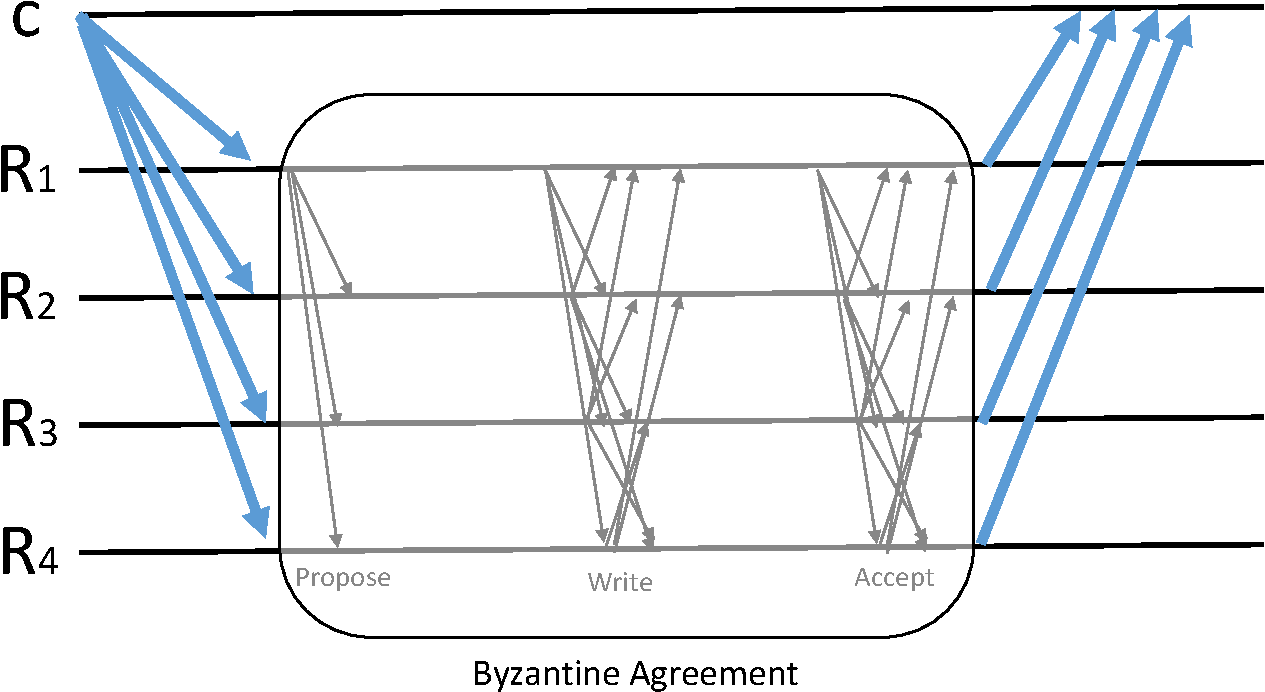
\includegraphics[width=.5\columnwidth]{images/images/bft.pdf}
\caption{Byzantine Fault Tolerance protocol overview.}
\label{fig:bft}
\end{center}
\end{figure}

The authors implemented \textsc{BFS}, a Byzantine fault tolerant Filesystem, to validate this \gls{bft} library. 
The results show that when the workload increases the throughput and latency is nearly the same of a non-replicated system. 
This level of performance encouraged the use of \gls{bft} in common systems, and to develop optimizations to improve \gls{bft} protocols. 
Since the \textsc{PBFT} proposal, some work has been dedicated to improve \gls{bft} protocols (see Table~\ref{tab:bft}):



\begin{table}[h]
\begin{center}
{\footnotesize
\begin{tabular}{ p{2.5cm}  p{10.5cm}  }\hline
\textsc{Zyzzyva}~\cite{Kotla:2010}  & Introduces speculation to avoid the expensive three phase commit before processing the requests. This might introduce some inconsistency in the state of the replicas when speculation fails, and the client needs to help replicas to fix the servers’ inconsistency. \\ \hline			
\textsc{Upright}~\cite{Clement:2009} & It provides a straightforward way to also add BFT to crash fault tolerant systems (CFT); \\ \hline	
\textsc{Aardvark}~\cite{Clement:2009b} & Shifts the paradigm to a new design. This design improves the performance under faulty scenarios trading some performance on the normal case; \\ \hline
\textsc{BFT-SMaRt}~\cite{Bessani:2014} & It is modular and multicore-aware. Supports replica reconfiguration and has a flexible programming interface; \\ \hline
\textsc{COP}~\cite{Behl:2015} & It is the most recent BFT implementation that reached 2.4 million operations per second. This was achieved mostly due to BFT architecture changes.\\  \hline  
\end{tabular}
}
\caption{Brief overview of the most relevant BFT works.}
\label{tab:bft}
\end{center}
\end{table}

\paragraph{Summary.} 
\gls{bft} replication has a major importance in this thesis. 
As we propose a control plane system that enhances \gls{bft} systems by adding intrusion tolerance mechanisms. 
We need \gls{bft} protocols to guarantee that replicas execute in the same order and to be able to tolerate some malicious failures in a subset of the replicas.
The implementation of such \gls{bft} protocol is a complex task, particularly if we need to include mechanisms for state transfer, reconfiguration, and guarantee a good performance.
Therefore, we prefer to rely on existent libraries than to build a new one.



\section{Replica Rejuvenation}
Software rejuvenation was proposed in the 90's~\cite{Huang:1993,Huang:1995} as a proactive approach to prevent performance degradation and failures due to software aging. 
The first proposals were based on periodical clean-up of the aging effects by restarting some parts of the software. 
This mechanism would postpone failures and restore the performance. 
This solution was implemented using three components: a watchdog process (\texttt{watchd}), a checkpoint library (\texttt{libft}) and a replication mechanism (\texttt{REPL}). 
A primary node executes the application and also runs the \texttt{watchd} to monitor the application crashes and hangs. 
The backup node, while the application is inactive, keeps monitoring the primary node. 
There is a routine (provided by \texttt{libft}) that periodically makes checkpoints and logging. 
These checkpoints are replicated with \texttt{REPL} in the backup node. 
When the primary node crashes or hangs, it is restarted, and if needed the backup takes his place on the execution.


Some years later, proactive recoveries where adopted on \gls{bft} replicated systems.
% \textsc{PBFT-PR}~\cite{Castro:2002} and \textsc{COCA}~\cite{Zhou:2002} introduced proactive recoveries in \gls{bft} replicated systems. 
Proactive Recovery is a mechanism that periodically rejuvenates the replicas to clean potential faults or stealth attacks. 
This mechanism allows that an adversary controls some replicas, usually $f$ , during a time window, where the system is vulnerable.

Castro and Liskov presented PBFT-PR~\cite{Castro:2002}, a \gls{bft} replication library that does proactive recovery. 
\textsc{PBFT-PR} assumes that replicas will frequently recover. 
Additional assumptions are needed to guarantee the \textsc{PBFT-PR}'s liveness and safety during the recoveries: 
(i) Each replica contains a trusted chip to store its private key, and it can sign and decrypt messages without revealing the key; 
(ii) The replicas’ public keys are stored in a BIOS read-only memory, which needs physical access to modify the BIOS; 
And last, (iii) a watchdog timer is used to avoid human interaction to restart replicas. 
The watchdog hands the execution to the recovery monitor, which cannot be interrupted.


Zhou~\etal{} presented \textsc{COCA}~\cite{Zhou:2002}, a fault-tolerant and secure online certification authority that has been built and deployed both in a local area network and on the internet.
\textsc{COCA} uses proactive signature sharing to ensure that when replicas fail and recover there is no key-leakage. 
Contrary to \textsc{PBFT-PR} it does not rely on trusted components, but it may need an administrator to refresh the \textsc{COCA} server keys.


Reiser and Kapitza~\cite{Reiser:2007} and Distler~\etal{}~\cite{Distler:2008} identified virtualization as a useful mechanism to implement proactive recovery in \textsc{VM-FIT}. 
The proposed architecture is divided in two domains an untrusted domain and a trusted domain.
The intrusion-tolerant replicated system executes in the untrusted domain, running in \gls{vm}. 
While \textsc{VM-FIT} executes in a trusted domain, i.e., in the \gls{vmm}. 
Virtualization allows the isolation between the untrusted and the trusted domains. 
Therefore, it can trigger recoveries from the trusted domain in a synchronous manner. 
Moreover, virtualization reduces downtime of the service during the recovery and makes the state transfer between replicas more efficient. 
The authors implemented this system using the Xen hypervisor to get the two domains: the trusted domain is the Xen Dom0, and the replicas run in the untrusted domains, DomUs.

Sousa~\etal{} improved the state-of-the-art recovery algorithms by introducing \gls{prrw}~\cite{Sousa:2010}. 
This technique removes the effects of faults ``immediately''. 
\textsc{\gls{prrw}} accelerates the rejuvenation process by detecting the faulty replicas behavior and forcing them to recover without sacrificing periodic rejuvenations. 
This type of technique can only be implemented with synchrony assumptions as the recoveries are time triggered~\cite{Sousa:2005}. 
To address this need the authors proposed an hybrid system model: the payload is an any-synchrony subsystem, and the wormhole is a synchronous subsystem. 
The authors implemented this system using the Xen hypervisor as the wormhole. 
Zhao~\etal{}~\cite{Zhao:2012} improved~\cite{Sousa:2010} with an algorithm to schedule the rejuvenations that is adaptable to a constant monitoring of the network and CPU/memory performance.


\paragraph{Summary.} \gls{bft} replication with proactive recovery represents one of the cornerstones of intrusion tolerance. 
Proactive recovery allows the system to reduce the vulnerability window of the replicated system drastically. 
\gls{bft} replication with proactive recovery guarantees the system's correctness while the replicas recover faster than $f+1$ replicas become faulty. 
One limitation of proactive recovery is that there must be a trusted element somewhere to implement this mechanism. 
Some works use hardware timers while others resort to virtualization to separate the execution domains. 
In our proposal, we will adopt an architecture similar to~\cite{Distler:2008} and~\cite{Sousa:2010}. 
However, our solution will implement a different (from~\cite{Sousa:2010}) algorithm to proactively trigger recoveries.
Most of these solutions assumed that replicas fail independently without addressing that issue. 
The following works address the failure independence through diversity. 


\section{Diversity}
In most of the works presented before, the correctness of the \gls{bft} is ensured under the assumption that replicas fail independently.
Therefore, they assume implicitly or explicitly that there is some mechanism that create different vulnerable surfaces which difficult the attacker's work.

Diversity can be implemented in different ways~\cite{Deswarte:1998,Obelheiro:2006}, which may differ in the mean and the amount of diversity generated, but the goal is the same: to create different attack surfaces (details in the survey~\cite{Baudry:2015}). 
The goal is to make the discovery of common vulnerabilities more difficult. 
We present at least three different ways to generate diversity: 
(i) N-version programming consists in design/implementation of different program binaries (from the same or different source code); 
(ii) Artificial diversity implements different memory or binary schemes; 
and (iii) Off-the-shelf diversity comprises the use of different products with the same functionality but taking advantage of implementations that are already available.

\subsection{N-version programming}
The first works on diversity were published in 1975, Randell~\etal{} introduced the idea of using different software design (i.e., implementations) as a way to achieve reliable software. 
By supplying a primary replica with a spare replica that would follow up if any failure is detected.

Chen and Avizienis~\cite{Avizienis:1977,Chen:1978} defined the notion N-version programming with the goal of achieving software reliability in redundant systems.
The principle was to defined N teams that would developed N versions of the same software specification that would be semantically equivalent.
Then, the N-version programs would execute, compare the outputs, if the outputs verify the equivalent condition then the it accepted.
These works opened a new area of security and reliability research.
Knight and Leveson made an empirical study that conclude that N-version must be employed with special care, as it for itself does not provide reliability guarantees.

\subsection{Automatic diversity}  
The idea of having to N different teams to develop N software versions did not seemed attractive, and sooner automatic approaches appeared.
Forrest~\cite{Forrest:1997} suggested randomized program transformations to introduce application diversity. 
They have made modifications on the gcc, a C compiler, in such a way that during the compiling time gcc inserts random padding
into each stack frame. 
%Linger presented stochastic diversification tool to swap code structures
The diverse versions are generated during the source code compilation. 
The main idea of these works is to make the intruder’s work more difficult when exploiting buffer overflow vulnerabilities.

Bhatkar~\etal{}~\cite{Bhatkar:2003} proposed a solution based on memory address obfuscation (i.e., \gls{aslr}). 
%Cox~\etal{}~\cite{Cox:2006} present N-variant system that uses automated diversity 
Their solution transforms object files and executables at the link-time and load-time, without kernel or compiler modifications. 
The goal is to ensure that an attack that succeeds in one target will not succeed on the other targets. 
Each time the program is executed its virtual addresses and data are randomized, and therefore the attacker needs to find new ways to exploit memory errors, like buffer overflows. 
However, a recent work proved that solutions like ASLR are vulnerable to attacks~\cite{Bittau:2014,Jang:2016}.
A few works propose the usage of compilers that generate different executables~\cite{Platania:2014,Roeder:2010,King:2016}.

Hoset and Cadar~\cite{Hosek:2015} proposed \textsc{Varan}, an N-version Execution framework.
\textsc{Varan} executes with a shared-memory ring among different processes (followers and one leader), these are launched by a coordinator that orchestrates and setups the execution environment.
Each follower runs a different rewritten binary only where there are system calls, this plays a big performance improvement when compared with other solutions.
The implementation of the memory ring is also a major improvements as it allows concurrent access by multiple producers and consumers.
The results show that some system calls when executed in \textsc{Varan} can introduce n overhead of 135\% when compared with a native setup.
The authors also scale out the number of followers, which, as expected, increase the overhead as they are added. 
\textsc{Varan} was purposed for reliability, however some principles could be adopted for security after solving some challenges, namely the use of the same address space that would benefit return-oriented programming.

 


\subsection{Off-the-shelf diversity}
The two previous solutions generate diversity before the software’s distribution. 
\gls{ots} diversity does not need pre-distribution of diverse mechanisms. 
It relies on the existence of different software components that are ready to be used.
There are plenty of different free products that provide the same functionality and were developed by different vendors. 
In other words, \gls{cots} diversity is like an opportunistic N-version programming.




\paragraph{Studies.}
Gashi~\etal{}~\cite{Gashi:2007} made an experimental evaluation of the benefits of adopting diversity of SQL database servers. 
The authors analyzed bug reports of four database servers (Post-greSQL, Interbase, Oracle, and Microsoft SQL Server) and verified which products were affected by each bug reported. 
They have found few cases of a single bug affecting more than one server. 
In fact, there were no coincident failures in more than two of the servers.
The conclusion is that \gls{ots} database servers’ diversity is an effective mean to improve system's reliability. 
However, the authors recognize the need for SQL translators, to increase the interoperability between servers in the replicated scenario.

Han~\etal{}~\cite{Han:2009} made a systematic analysis of the effectiveness of using \gls{ots} diversity to improve system's security. 
First, the authors found if there were \gls{ots} software substitutes to provide the same functionality. 
Then, they determined if the \gls{ots} software shared the same vulnerabilities.
And if so, if the same vulnerability could be exploited with the same attack. 
In this study, more than 6k 1 vulnerabilities were analyzed, which were published in the \gls{nvd} on the year 2007. 
The results showed that 98.5$\%$ of the vulnerable software have substitutes. 
Moreover, the majority of them either did not had the same vulnerabilities or could not be compromised with the same exploit code. 
It is not expected that a single exploit works in different \glspl{os} because each one has a different memory scheme and different filesystems. 
Even between versions from the same \gls{os}, the low-level functions change across the versions. 
The study also concluded that 22.5$\%$ of the vulnerabilities were present in multiple software. 
However, only 7.1$\%$ from those vulnerabilities were present in software that offers the same service. 
The study findings are a good sign that diversity can improve a system’s dependability.


Garcia~\etal{}~\cite{Garcia:2014} studied the vulnerabilities among \gls{ots} \glspl{os}. 
Similar to \cite{Han:2009} this study was carried out taking vulnerability feeds from \gls{nvd}. 
However, this work was only focused on \glspl{os}, and the data collected comprised 11-year of vulnerability reports. 
Our goal was to find to what extent different \glspl{os} shared common vulnerabilities. 
In this study, we analyzed 2270 vulnerabilities entries manually, where they were classified in different categories. 
Then, we defined three types of servers: (i) a server that contains most the packages/applications available (Fat server); (ii) a server that does not contain unnecessary applications to a certain
service (Thin server); and (iii) a thin server but with physically controlled access (Isolated hin server). 
We assumed that the third setting it is the most advisable for critical systems, since additional care is taken to install and setup its configuration. 
For each configuration, we compared all the common vulnerabilities in pairs of \glspl{os}. 
As expected, in the Isolated thin server, the number of common vulnerabilities was considerable less than in the other configurations. 
There was only 1 vulnerability that was shared among six \glspl{os}, 2 that were shared among five \glspl{os}, and 130 that are shared between two \glspl{os}. 
We went further in the study and looked for common vulnerabilities in different versions of the same \gls{os}. 
We have found evidence that suggests that using OS diversity in a replicated system can improve its dependability. 
Even if few \glspl{os} are employed, it is possible to achieve vulnerability independence just with different versions.


Larsen~\etal{} made a study with several examples on how to apply diversity~\cite{Larsen:2014,Larsen:2015}. 
The paper explains in detail what to diversify, from single instructions to an entire program. 
They also explain the three types of security impacts when diversity is applied: entropy analysis, attack-specific code analysis, and logical argument. 
However, they also point that there is no consensus on how to evaluate the efficacy of diversity. 


Zhai~\etal{}~\cite{Zhai:2014} propose a system that looks for independence failures from the reliability standpoint on the cloud.
The system collecs and audits data from the system components to evaluate its components' independence identifying potential correlated failures.
The authors collect information on networkd, hardware, and software data.
Then, the different configuration dependency are analyzed and ranked in risk groups as a way to see how the different dependencies may make the system fail.
The main limitation of this work is the motivation that clouds may not have to join such system, i.e., provide private data to be analyzed for external agents.
The experimental evaluation is concerned to the time that it takes to analyze all the data and creating the dependency graphs.
CITAR COM ESTE~\cite{George:2015}




%Network diversity 
\paragraph{Network diversity.}
Newell~\etal{}~\cite{Newell:2015} presented a solution to assign diversity variants among network nodes to increase the network's resiliency (in particular its connectivity).
The authors present this as a Diversity Assignment Problem, although it is an NP-hard problem the authors show that for medium-size random networks graphs it is feasible.
For medium-sized networks they use mixed-integer programming and for larger networks propose a fast greedy approach.
For the first one the achieve optimality, and the latter an approximation of the optimal.
One of the results that the authors show is that random diversity assignment is far worse than an criteria assignment (as they propose).
Despite the different results that show improvements of diversity on the connectivity (i.e., resiliency), the models did not used realistic data, thus the authors assumed that the compromise values are known and independent with each other.


Zhang~\etal{}~\cite{Zhang:2016} propose a metric to evaluate the resilience of networks.
The idea is to define what is the least attacking effort to compromise some important assets of the networks (i.e., this work is focus on distributed yet not replicated systems).
Therefore, they measure the weakest path to target and compromise the main asset. 
The authors proposed three metrics which where evaluated in a simulated environment.
None of the three metrics uses vulnerability data to correlate the existence of common weakness, on contrary, the metrics use data about the topology, services installed, etc.
Nevertheless, the results show that increasing the diversity on the nodes reduces the number of simulated worms.
 


\paragraph{Summary.}
We presented three different techniques that support diversity as a fault-tolerant mechanism. 
N-version programming is the most costly, since it needs different developers or additional programs to verify if the automatic translation works. 
On the contrary, \gls{ots} and randomization diversity are almost for free. 
The first one can be obtained from free sources that are ready to be used, and the second one is automatic and already supported
in most OSes. 
Diversity still has some gaps that must be addressed to make it an effective building block of intrusion tolerance. 
For example, how to measure diversity in such a way that failure independence can be guaranteed?


\section{Practical Systems with Diversity}

Totel~\etal{}~\cite{Totel:2005} proposed an \gls{ids} based on design diversity.
The authors described an architecture that uses a set of replicated \gls{cots} servers, a proxy, and an \gls{ids}. 
The proxy is responsible for forwarding the requests from the client to every \gls{cots} server. 
When the servers reply, the proxy sends the responses to the \gls{ids} to be analyzed. 
The IDS compares the responses from the \gls{cots} servers and if it detects some differences an alarm is raised. 
Then the proxy votes the responses and replies to the clients. 
The authors developed an algorithm to detect intrusions and tested their solutions against Snort~\cite{snort} and WebStat~\cite{Vigna:2003}. 
The results show that using diverse-\gls{cots} service (e.g., http) allows the \gls{ids} to deliver fewer alarms without missing the intrusions.

Bairavasundaram and Sundararaman~\cite{Bairavasundaram:2009} implemented \textsc{EnvyFS} a filesystem that uses N-version filesystems implementations to guarantee the reliability of stored data.
Their solution is able to tolerate filesystem mistakes (e.g., crash, integrity).
To keep the system simple, the authors used a virtual filesystem layer that abstract the specific filesystems underneeth, therefore some challenges arise from the different implementations details.
Another challenges, was to avoid the need for multiple storage as it uses N-variants of filesystems. 
However, they solved this by using the only one storage layer and the different filesystems in between. 
Then, after each filesystem executes the commands a voter collects the majority of outputs to store.
The results show that EnvyFS is able to improve the reliability by leveraging on multiple filesystems.
However, the performance results show that EnvyFS pays the price of executing in multiple filesystems and waiting for a majority of them. 
In most of the time it takes the sum of the three filesystems used.

Diversity has also been adopted to work a malware detector. 
Xu and Kim~\cite{Xu:2017} introduced \textsc{PlatPal} that analyzes the behavioral discrepancies of malicious document files on different platforms (e.g.,Windows or Macintosh). 
\textsc{PlatPal} loads a file in both systems and monitors the execution traces/or crashes. 
In the end, both systems compare the outputs, if divergences are observed it is signaled an attack.
The authors focused on a particular application, Adobe Acrobat Reader, it reads pdf files which a standard format, and both \glspl{os} have the application available.
Therefore, besides the internal discrepancies the correct executions should be very similar.
There are some limitations, namely is fails to detect social engineering attacks or attacks that need some human interaction.
Although \textsc{PlatPal} is proposed to detect malicious payloads on files, it vouches (indirectly) for diversity as it shows that an attacker needs to deploy multiple payloads to compromise the the system with the same attack (for the majority of the malwares samples used).

(see ~\cite{Yuan:2014} for a survey)


\textsc{BASE}~\cite{Rodrigues:2001} is an extension of PBFT~\cite{Castro:1999} that explores opportunistic \gls{ots} diversity in \gls{bft} replication. 
The system provides an abstraction layer for running diverse service codebases on top of the PBFT library.
The key issue addressed by BASE is how to deal with different representations of the replica's state, allowing a replica that recovers from a failure to rebuild its state from other replicas. 
BASE was evaluated considering four different OSes and their native \gls{nfs} implementations: Linux, OpenBSD, Solaris, and FreeBSD.
The results, from 16 years ago, show the same trends we observed: performance varies significantly when diversity is considered.
Differently from \system, \textsc{BASE} does not address the selection of replicas or the reconfiguration of a replica group.

In order to support long-running services, Castro and Liskov~\cite{Castro:2002} introduced the notion of proactive recovery for \gls{bft} services. 
The objective is to rejuvenate replicas periodically to remove stealth attackers and support the execution of long-running services. 
All works on \emph{safe} proactive recovery consider the use of trusted local component on each replica to trigger the periodic recoveries~\cite{Castro:2002,Sousa:2010,Roeder:2010,Platania:2014,Distler:2011}.
%, and some of them even support reactive recoveries to deal with service degradations caused by detectable attacks~\cite{sousa:pc}.
A common weakness of most of these works is that they do not support diversity, therefore a compromised replica can be attacked immediately after its recovery by exploiting the same vulnerability.
The two noticeable exceptions are discussed in the following.

Wang~\etal{}~\cite{Wang:2003} proposed an architecture, named \textsc{SITAR}, which aims to build intrusion-tolerant systems with diversity and dynamic reconfigurations.
It works in front of \gls{cots} server that are vulnerable, thus needing additional protection mechanism provided by \textsc{SITAR} in a form of proxy servers that have publicly access to the exterior.
These proxies receive the requests audit them based on the current threat level, then they propagate to acceptance monitors if they pass the accepting test they are delivered to the \gls{cots} servers. 
In the way back, the acceptance monitors validate the response and run an agreement protocol to select a final response from the \gls{cots} servers.
There is a adaptive reconfiguration module that monitors the other modules, receiving heartbeats and intrusion triggers to take action on removing compromised modules and starting new ones.


Arsenault~\etal{}~\cite{Arsenault:2007} presented a \gls{scit} a centralized architecture to support node cleansing inside a cluster.
\gls{scit} goal is to clean the elements of a cluster without harming the availability of the overall service.
Recovering the clusters nodes allows for reseting the state and avoiding huge windows of vulnerability on the nodes.
Nevertheless, the \gls{scit} service itself can be harmed, therefore the authors leverage on trusted hardware to offer additional guarantees to the system.
The architecture supported by trusted hardware and full isolation allows \gls{scit} to operate in predictably and continuously manner regardless the presence of attacks.


Roeder and Schneider~\cite{Roeder:2010} propose an intrusion tolerance technique called \gls{po} for supporting a different type of diversity from \system.
The idea is, instead of changing \glspl{os} or other off-the-shelf component of the replica, \gls{po} changes the application and library code periodically preserving the original semantics using program transformations, i.e., system call obfuscation reordering, memory randomization, and functions return checks (through an IBM \textit{gcc} patch that inserts and checks a random value after the functions return).
Each replica generates its own obfuscated executable from a read-only device containing the ``master code'' based on time-triggered epochs that a controller triggers in a secure way through a trusted component similar to \system' \gls{ltu}.
All obfuscation mechanisms were implemented and evaluated on OpenBSD 4.0, and their results show that PO adds a little extra overhead to the non-\gls{po} execution.

Similarly to \gls{po}, Platania~\etal{}~\cite{Platania:2014} proposed a compiler-based diversity for the Prime \gls{bft} protocol~\cite{Amir:2011} using the MultiCompiler tool~\cite{Homescu:2013}. 
This compiler creates diverse binaries from the same source code through randomization and padding techniques.
The authors also proposed a theoretical rejuvenation model that receives as input: the probability of a replica being correct over a year ($c$); the number of rejuvenations per day across the whole system ($r$); the number of replicas ($n$); and the system's lifetime. 
Although operators can control only $r$ and $n$, the authors suggest (but does not show how) that $c$ can be estimated using \gls{osint} from the internet (CERT alerts, bug reports, and other historical data).
The authors implemented their solution in two settings, including a virtualized environment provided by the Xen Hypervisor.
In this setting, each replica executes in a Linux \gls{vm}, the recovery watchdog runs in a trusted domain of the same machine, and the proactive-recovery controller runs in another physical machine, in an architecture similar to ours.


\paragraph{Summary.} 
Diversity is becoming one of the building blocks of intrusion tolerance, alongside with \gls{bft} and rejuvenations. 
We presented few works that already used somehow diversity in intrusion-tolerant systems. Some of the works employed opportunistic \gls{ots} components to create diversity among the replicas. 
We do not discard the possibility of using other diversity techniques, such as randomization. 
However, in our work we are interested in \gls{ots} diversity because it is possible to estimate the vulnerability of each component. 
These works are still limited to that extent, i.e., there are none or few concerns on how to create diversity to avoid common failures. 
Most of the works implement diversity assuming complete fault independence, but that is unrealistic. 
For example, different \gls{ots} \glspl{os} can share the same weaknesses due to some shared libraries or kernel code. 
There is a need to understand how diversity can be efficiently employed in a replicated system to make the failure independence sound. 
Moreover, further work is still necessary to create automatic mechanisms that abstract diversity management for the administrators.



\section{Vulnerability Analysis and Risk Management}

Bilge and Dumitras~\cite{Bilge:2012} made a systematic study on zero-day attacks between 2008-2011.
In their study, the main dataset is \gls{wine} (developed by Symantec), it sample and aggreates data from several hosts running Symantec products (e.g., Norton Antivirus).
The \gls{wine} data is correlate with \gls{osvdb} and Symantec's Threat Explorer for attack/exploit information.
Their method allowed them to measre the duration of zero-day attacks, the average attack lasts ten months. 
Moreover, they have found that some of the vulnerabilities exploited during the Stuxnet attack have been employed two years before Stuxnet in another attack.
One of the main conclusions of this work is the evidence that the disclosure of zero-day vulnerabilities increases the risk, up to five orders of magnitude, of users being attacked.
The vendors are responsible to prioritize the disclosure of such vulneraiblities and prepare a patch as soon as possible. 


%% RISK ASSESSMENT (DISTRIBUTED) NETWORKS 
Poolsappasit~\cite{Poolsappasit:2012}~\etal{} propose a security risk assessment method that incorporates the cause-effect relationships of the network states and the likelihood of exploiting such relationships.
To do that, they measure the organizations security risk using \gls{cvss} metric.
The authors implemented a tool that generates a map of the network as a Bayesian attack graph, then it collects data with a vulnerability scanner and it fetches the vulnerability exposures for each vulnerability.
The result is helpful for system administrators that can have an overview of the network weaknesses and associate a cost to the assets in a way that countermeasures can be taken to avoid such weaknesses.
The countermeasures are indicated by the system administrator that will link them to the attributes model.
Then, the administrator assign the damage costs to every attribute.
Finally, a genetic algorithm will evolve the network for states that the cost of losing assets (i.e., being compromised) is minimal. 
Their empirical results show that they can minimize the costs of being compromised by assessing the security of the system and applying the most cost-efficient countermeasures.
Besides the manual setup that the system administrator needs to perform, it would be interesting to see how fast the system can react once an attack is detected.


EDIT: Why we dont addopt these techniques to the Bft domain? Mapping an entire organization network comprises an infinity of attributes and implication relationships.
In our case, we are mostly focused on the 3f+1 fault model, therefore, to achieve dependable goals with such fault threshold we are only concern with what causes can make $f+1$ being compromised.


Nappa~\etal{}~\cite{Nappa:2015} analyzed the patch deployment process over 10 popular client applications on a 5-year period, in some cases, wich applications share libraries, the patching process takes different time to the same vulnerable shared code. 
The authors have found that there is a strong correlation between the vulnerability disclosed and the start patching process among vendors, for 77\% of the studied vulnerabilities it occuers within seven days. 
The performed a \emph{survival analysis} (inspired in medicine and biology to measure the mortality rates associated with diseases) to measure the probability a vulnerable host will remain vulnerable beyond a specific time.
The vulnerability ''dies`` once a patch is installed or a non-vulnerable software is installed.
The experimental results show that using real-wordl WINE exploits still compromise 50\% of the vulnerable hosts (after vulnerabilities discloser). 
The median percentage of hosts that have been patched before the exploit is released is at most 14\%.
Together with the number of shared vulnerable code with different patching delays, these values motivate attackers to re-used already know exploits or to create patched-based exploits~\cite{Brumley:2008}.
The authors also show evidence to support the natural intuition that silent or automatic updades reduce the survivavility of vulnerabilties. 
They also, performed an analysis on three different user profiles that show that security analysts are more cureful on patching software than software developer or normal users.

Jumratjaroenvanit and Teng-amnuay~\cite{Jumratjaroenvanit:2008} described vulnerability life-cycles presenting their different stages. 
The authors goal was to understand how different dates can be useful to estimate the probability of an attack. 
The authors methodology was to collect and analyze data on the discovery, disclosure, and exploit dates, exploit and patch availability, all from public data sources. 
They used this information to define five life cycle types: (i) \gls{zda}, which typically is a done by a black-hat and is defined by the date of disclosure and exploit being the same; (ii) \gls{pzda}, is a \gls{zda} but with a patch already available, but not applied; 
(iii) \gls{ppzda}, is a \gls{pzda} but does not matter if the patch is available or not; 
(iv) \gls{poa}, it is a zero-day vulnerability. 
The most influential variables were the code that was scrutinized by a the tester with access to the source code, and the code that was analyzed with some static tool before. 
On the contrary, results showed that language safety was the less influent factor. 
The main result of the study was that two weeks of work were enough to have a 50\% chance of finding a zero-day vulnerability. 
Sometimes, 53 hours were enough to find one vulnerability with more than 95\% of probability.


Frei~\etal{}~\cite{Frei:2010} made a quantitive analysis of 27K vulnerabilities disclosed in the last decade.
The authors propose a model that describe the main players in a vulnerability lifecycle.
All the dates associated with the vulnerability lifecycle are described in details before the analysis.
They used a few public vulnerability databases (e.g., \gls{nvd} and \gls{osvdb}) to collect the different data attributes.
The results show that the number of patches increase after vulnerability disclosure.  
One interesting result is the \emph{the gap of insecurity} measurment, where they compare the patch availability vs the exploit availability. 
The results show that exploits are always ahead of patches, in some cases after 30 days of disclosure the number of exploits exceeds 90\% the number of patches.


Bozorgi~\etal{}~\cite{Bozorgi:2010} used machine learning techniques to classify existent vulnerabilites and predict future exploits.
Their results show that their trained classifiers outperform current exploitability measures like \gls{cvss} exploitability subscore.
They have built a dataset with two public databases Mitre' \gls{cve} (which is subpart of \gls{nvd}) and \gls{osvdb}.
They used the bag-of-words, a machine learning technique, to extact the textual attributes that are more relevant to analyse.
They used \gls{svm} to train the model, to conduct two types of experiments: an offline and an online.
In the offline setting, which they train and evaluate data in a static fashion, they achieve an accuracy of 90\% of correct predictions.
In the online settting, the results show that after a small period the model stablizes and reduces the overall error by 14\%.
In an online setting they were able to make preditions up to two days before the exploit with an accuracy of 75-80\%.
The main result, for the interest of this thesis, is the comparison between their model and the \gls{cvss} as a measure of indication of how a vulnreability is likely to be exploited.
The \gls{cvss} attributes high scores to vulnerabilities that were not exploited. 

Allodi and Massacci~\cite{Allodi:2014} made a in depth analysis of four security databases (e.g., \gls{nvd}, Exploit-DB, SYM, and EKITS). 
The authors made a in deph \emph{break down} of \gls{cvss} on its several attributes, for example, exploitability the subscore \emph{resembles more a constant than a variable}, thus not have a real impact on the \gls{cvss} score.
They used a randomized case-control study, which is applied to different study domains.
Is used to assess the effectiveness of a treatment over a sample of subjects.
In this study in particular the want to measure how \gls{cvss} influences the \emph{risk factor} of the studyie cases.
A result that is worth of note is that fixing vulnerabilities based on their \gls{cvss} is statistically equivalent to picking a random vulnerability to fix, from the security relevance standpoint.
On contrary, the authors suggest that it is more important to fix vulnerabilities that appear in the black market of vulnerabilities.
Their results indicate that the inclusion this information as a \emph{risk factor} can increase the risk redcution up to 80\%.
The authors point that EKITS datasource may be a threat to the validity of the study, as it is unstructured data and therefore it requires manually anaylsis.

Sabote~\etal{}~\cite{Sabottke:2015} presented a study that used non-common vulnerability data sources, i.e., Twitter data (e.g., specific words, the number of retweets, and replies, information about
the users posting these messages), to find exploit data. 
The authors made a quantitative and qualitative exploration of the vulnerability-related information disseminated on Twitter.
They developed a Twitter-based exploit detector to provide an adequate response in a such short time frame. 
This allows the security community to foresee the exploit activity before the information reaches the de facto disclosure data sources like \gls{nvd} and ExploitDB.
However, to complement and strength their information results they also used sources like \gls{nvd}, \gls{osvdb}, Exploit-DB, Microsoft Security Advisories and Symantec WINE. 
The authors distinguished the real-world exploits from the proof-of-concept exploits, as the latter are by products of the disclosure process. 
The real-world exploits typically are not known until a critical zero-day attack occurs. 
The authors used \gls{svm} to classify exploits in the social media and tested how robust it was to attacks, i.e., if a powerful attack could manipulate the information on Twitter with a false account and false data. 
The results showed that with their proposal they could be confident with the predictions. 
For example, the \gls{svm} classifier set to a precision of 25\% could detect the Heartbleed exploits within 10 minutes of its first appearance on Twitter. 
They also showed that organizations like \gls{nvd} overestimate the severity of some vulnerabilities that never become in fact exploited.
However, their work did not focus on the discovery of the zero-day vulnerabilities, which is relevant for our research.



Shahzad~\etal{}~\cite{Shahzad:2012} obtained data between 1988 to 2011 from three data sources: \gls{nvd}, \gls{osvdb}, and the data from~\cite{Frei:2006}. 
They collected vulnerabilities that affected popular applications like Internet Explorer, Firefox and Chrome, and popular \glspl{os} like Windows, Mac OS X, Solaris and several Linux distributions. 
The authors found that 2006 was the peak of vulnerability disclosures, and since then there was a decrease even though there are more software products. 
However, the complexity of the disclosed vulnerabilities has increased, ased on the \gls{cvss} score. 
From their dataset, 2.8\% vulnerabilities have an exploit released before their public disclosure. 
More dramatic is the percentage of exploits that are released on the day of the vulnerability disclosure, which is in the order of 88.2\%. 
There are a cases when even after the disclosure there are exploits being released (the authors found 9.7\% of their vulnerabilities fitting this condition). 
As already stated in~\cite{Gorbenko:2011}, the software’s popularity can be attractive to attackers. 
In this study, the authors found that Microsoft and Apple have more exploits before the vulnerability disclosure than the other vendors. 
This may primarily be because hackers find it more rewarding to exploit these products due to their wider market capitalization.
To what concerns patching, the authors argue that 10\% of the vulnerabilities had a patch before their disclosure, and 62\% had a patch on its disclosure day. 
There was a considerable number of vulnerabilities that were disclosed only after a patch is made, more precisely 28\%. 
However, the authors noticed that from 2007 there was an improvement from the vendors to respond to vulnerabilities with earlier patches. 
Nevertheless, the closed-source vendors are more efficient to patch vulnerabilities. 
Another conclusion is that it is easier to exploit opensource code vulnerabilities than in closed-source – this conclusion may seem obvious, but no one had showed it previously with statistical tests.


Holm~\cite{Holm:2014} made an analysis malware alarms to verify if there is a statistical distribution to model the number of intrusions or the time to compromise a computer system.
The author collected information from different software configurations from 2009 to 2012 from an IT enterprise.
The enterprise had a total of 697 \glspl{os} versions.
Each computer is equipped with an anti-malware software, when a malware is detected it sends the data to a central database.
The author's methodology applied a few filters to reduce the size of the data by removing redundant information (e.g., a single malware can generate several alarms in the systems).
The results show that the Pareto distribution is the one that best fits for the time of the first compromise.
Another interesting result is that the more the system is intruded the more vulnerable it is. 
The authors present some hypothesis for this result, for example, once the system is broken it can no longer be trusted, but it seems odd to conclude something about how vulnerable the system is. 
A more plausible one is that the security awarness in only temporary increased as a result of the intrusion, and then it is again neglected.
Most of the malware considered in this study were not result of targeted attacks but rather automatic ones, this is probably due to the type of enterprise. 
This may change the results if applyied to targeted attacks as they require a different strategy to penetrate the system,.


%data analysis
Massacci and Nguyen~\cite{Massacci:2010} made an analysis of several datasources that provide data about vulnerabilities, exploits and patches. 
The authors raise some limitations on the datasources, namely the difficulty to map some of the listed sources. 
However, it is possible to use the \gls{nvd} mappings that provide code mappings for \gls{cve} and the respectively ID from the other datasource.


Guo and Bhattacharya addressed the problem of \gls{bft} replicas fault independence~\cite{Guo:2014}.
The authors proposed different replicas configurations using \gls{ots} \glspl{os} to increase the diversity among the replicas. 
There was a set of different configurations that could build a replicated system. 
Each configuration was composed of different \gls{os}. 
The authors proposed a formalization of the virtual replica diversification problem. 
They used a game-theory approach to find an optimal diversification strategy for the defender's side. 
The authors validated their model with the \gls{nvd} data used in~\cite{Garcia:2012}.

Wang~\etal{} proposed a different approach to measure the risk~\cite{Wang:2014}. 
Contrary to the most common approaches that attempt to measure the vulnerability state of the syste, the authors explored how many zero-day vulnerabilities were required to compromise a network. 
They address diversity, however, as replication is not considered the use of diversity in a ''chained`` archictecture will no enhance the system's security.
One of the limitations of this approach is that it considers all zero day vulnerabilities equally likely to happen.
Moreover, the metric's calculatation is complex and no evaluation is provided to hint the reader on how long can it take to calculate.
A similar work is proposed in~\cite{Bopche:2015}.

%Similar to ours, but very weak.... need to read and show how it fails~\cite{Mu:2014}


Gorbenko~\etal{}~\cite{Gorbenko:2017} used \gls{cve} and \gls{nvd} databases to study vulnerability life-cycles of differnet \glspl{os}.
The authors made a particular effort to analyze the relation between vulnerabilities' discovery and their fix, more precisely the time it takes to vendors patch the vulnerable software.
Moreover, they also studied the existent of common vulnerabilities among different \glspl{os}.
The resuls of their study show between 2012 and 2016 most of \glspl{os} used in their study patched every vulnerability that was disclosed in that period, with the exception of Ubuntu Server 12.04.
Another interesting result are the results for \emph{forever-day vulnerability} (i.e., vulnerabilities that are publicly disclosed but not yeat patched). 
They show that, for the analyzed period, Ubuntu never had a single day free from vulnerabilities, and Windows and Red Hat had  only 12 and 10, respectevily.
However, the most important results is the implications of \gls{cvss} on the \emph{days-of-gray-risk} (i.e., the number of days it takes to a vendor releases a patch). 
The authors show that there is no obvious implication on the level of severity and the time it takes to a vendor develop a patch.


\paragraph{Summary.} We presented several works that carry out for risk assessment in a way to prevent exploits or to take action upon vulnerability detection. 
This is the last building block that intrusion tolerance is missing. 
There is a lot of relevant free information available to address the security and dependability of software. 
In a replicated context this information is even more relevant. 
First, to react upon vulnerability/exploit disclosures, and second to select what configurations are less vulnerable to common weakness. 
We want to explore the free available data to improve, the dependability and security of intrusion-tolerant systems, by ensuring the assumption of failure independence with evidence supported by  relevant data.
A few works in different goals than ours did analyze vulnerability textual data~\cite{Joshi:2013} -- citar mais tarde



\section{Informed Diversity Systems}

Junqueira~\etal{}~\cite{Junqueira:2005} proposed \emph{informed replication} an approach to design distributed systems that can survive to catastrophes.
Their proposal focus on the diversity selection of the components a way to avoid common pathogens that compromise the whole system.
The authors propose a new system model that maps different software in attributes of a node, thus this attributes represent characteristics that should be distinct on each node to avoid common failures.
While modeling the system some biases are introduced, namely, considering that two different services that use the same port are vulnerable to the same vulnerability, or that the same service running with two different ports do not.
They propose an heuristic to build configuration in linear time.
Its goal is to distribute the \glspl{os} and applications in different configurations in such a way that minimizes the number of common attributes that would compromise the configuration.
They propose two metric a uniform that selects \glspl{os} uniformly and a weighted that selects \glspl{os} on their popularity.
The results show that their solution mitigates the number of pathogens that can compromise an entire configuration as its attributes are selected in order to maximize their difference.
The heuristic guarantee 0.99\% probability of data survival on attack of single- and double-exploit pathogens while needing only 3 and 5 copies respectively.



Seondong~\etal{}~\cite{Seondong:2017} propose a system that uses data from \gls{nvd} to select the best configurations of diverse \glspl{os} and web servers.
This is the work that most resembles one of the main contributions of this thesis. 
\side{**NOT TOP**}The algorithm they propose minimizes the \gls{cvss} of shared vulnerabilities among the different software.
Although they their experiments explore different configurations of software stacks, the decisions are based on the \gls{cvss}.
All the experiments were made in a simulator (i.e., CSIM 20) which difficult a fair analysis of performance evaluation. 
Moreover, the resilience of the system was evaluated against \gls{dos} attacks that affect particular vulnerabilities in the software used.
Depending on the type of the \gls{dos} it can cause performance decreases without exploit a vulnerability, and from the \gls{bft} standpoint compromising $f$ replicas is enough to compromise the whole system.
In other words, \gls{dos} evaluation does not show if $f$ is compromising the security and dependability properties besides the availability to some extent. 



%% MOVING TARGET ATTACKS
Okhravi~\etal{} presented \textsc{TALENT} a framework for live migration of critical infrastructures across heterogeneous platforms~\cite{Okhravi:2014,Okhravi:2012}. 
The idea was to create a moving target that difficult the success of advanced targeted attacks. 
TALENT implements OS level virtualization with containers, which allows the system to migrate the OS between machines periodically or upon detection of malicious activity. 
The virtualization was implemented with OpenVZ and LXC for Linux, Virtuozzo for Windows, and Jail for FreeBSD. 
The network was also virtualized, more precisely, a second layer of virtualization was used to migrate the IP address from one container to another. 
Even an established ssh session was preserved during the migration. 
Additionally, the state of the application also had to be migrated by employing a checkpointing technique. 
When all the programs were checkpointed, the state was saved and then was migrated by mirroring the filesystem. 
The filesystem synchronization took 98.7\% of the migration time. 
The authors decided to focus on optimizing the filesystem synchronization. 
In the optimized version, the filesystem synchronizes in periodic intervals by sending the differences to the destination. 
Therefore, the migration was made seamless to the application. 
TALENT also had a risk assessment, called operation assessment, which monitored and adjusted the diverse components using vulnerability information. 
However, there was almost no details on how the risk was measured and on how to adapt to the threats in an efficient manner.

Hong and Kim~\cite{Hong:2015} classified \gls{mtd} into three categories (e.g., shuffle, diversity and redundancy) and assess the effectiveness of each one.
The authors integrated the three solutions in \textsc{HARM} and evaluate how each technique improve the security of distributed systems.
The solution is built on top of \gls{vm}, as each \gls{vm} is able to host a few \glspl{os} in it.
Then, the evaluation scenarios consider three hosts running from two to three \glspl{vm} inside.
The three techniques were evaluated separately and they consider only two \glspl{os} on the diversity evaluation.
In the presented scenarios, deploying random diversity does not improve the risk of the system, but according to their results employing diversity have some trade-offs while it may break the connectivity between clients and servers (i.e., in their architecture ideally each host should have at least one \gls{vm} with diverse \gls{os}, otherwise, one host can be attacked and lose connectivity to the others).
However, these results are not surprising if only two \glspl{os} are considered. 

\paragraph{Summary.}



\section{Final Remarks}
In this chapter, we described the most relevant works that are related to this thesis.
We have made background revision of the intrusion-tolerance area, then we described the different topics that support to intrusion-tolerant systems.
Our main contributions are on the management of \gls{bft} systems, in particular, how to create diverse replica that effectively are independent and when the replicas need to be recovered. 
Although we could adopt solutions from artificial diversity, besides identified limitations~\cite{Snow:2013,Bittau:2014}, we are more interested in \gls{ots} diversity.
\gls{ots} diversity allow us to use data to make decisions on which diverse options work better together.
Such decisions would take action as rejuvenation triggers. 


%\system exploits the opportunistic \gls{ots} diversity derived from the existence of many version for \glspl{os}, \glspl{db}, Web Servers, \gls{jvm}, etc.
%Several studies show that different versions of these components significantly increase chances of avoiding common-mode failures~\cite{Gashi:2007,Garcia:2014,Gorbenko:2011}.
%Although we focus only on OSes in our \system prototype, the same techniques can be used to evaluate and deploy full diverse software stacks in the replicas.







